\documentclass[11pt]{report}
\usepackage[utf8]{inputenc}
 \usepackage{listings}
 \usepackage{color}
 \usepackage{fancyhdr}
 \usepackage{graphicx}
\pagestyle{fancy}

 \lhead{Geoffrey PERRIN \\ Océane DUBOIS}
 \rhead{MI01 - TP03 : VHDL séquentiel temporisé}
 \rfoot{}



\definecolor{dkgreen}{rgb}{0,0.6,0}
\definecolor{gray}{rgb}{0.5,0.5,0.5}
\definecolor{mauve}{rgb}{0.58,0,0.82}

\lstset{frame=tb,
  language=vhdl,
  aboveskip=3mm,
  belowskip=3mm,
  showstringspaces=false,
  columns=flexible,
  basicstyle={\small\ttfamily},
  numbers=none,
  numberstyle=\tiny\color{gray},
  keywordstyle=\color{blue},
  commentstyle=\color{dkgreen},
  stringstyle=\color{mauve},
  breaklines=true,
  breakatwhitespace=true,
  tabsize=3
}


%Gummi|065|=)
\title{\textbf{TP03 - Prise en main de l'environement de développement assembleur et premiers programmes }
\author{Geoffrey PERRIN \\ Océane DUBOIS\\}
\date{}}

\begin{document}

\maketitle

\newpage

\section{Exercices : affichage de chaîne de caractère}

\subsection{Programme "Hello World"}

Dans le fichier "hello1.asm", la variable msg est définie comme un suite de bytes contenant "bonjour tout le monde".
La variable longueure est définie comme un data double word (il occupe ainsi tout un registre) contenant la valeur 21 soit le nombre de caractères (occupant chacun un byte) de la chaîne de caractère msg.

Le programme fonctionne donc ainsi :
\begin{itemize}
\item La fonction main (seule fonction du programme), commence par réaliser une sauvegarde pour le code 'C' grâce à push ebx (le contenu de ebx est mis sur le sommet de la pile)
\item puis le registre ebx est mis à 0
\item puis on définie la ligne de programme qui suit avec l'étiquette "suivant". Cet ligne permet de mettre dans eax le contenu de l'adresse pointée par la somme de ebx et l'adresse de message. Le reste du registre sera completé par des zéros. Ebx va ici nous servir de controleur pour le nombre d'itération effectuées.
\item puis on met sur la pile le caratère à afficher et on appel la fonction c "putchar" qui elle-meme appelle fputchar qui permet d'afficher le caractère qui à été mis sur la pile.
\item puis on ajoute 4 au pointeur de pile pour le déplacer sur un emplacement non encore utilisé par le programme
\item on incrémente ensuite notre itérateur ebx
\item on effecture la comparaison entre ebx et la valeur contenue dans la variable longueure, les drapeaux sont mis à jour
\item si ebx et la valeur de longeur ne sont pas égaux cela signifie qu'on est pas arrivé à la fin de la chaine de caractère, on retourne donc à la ligne du programme ayant comme étiquette suivante et on réalise cette boucle jusqu'a ce que la valeur de longueure soit égale à la valeur de ebx.
\item si ebx et le contenu de longueur sont égaux on peut appeler la fonction c getchar qui attent l'appui sur "Entrée"
\item on met le sommet de la pile dans ebx
\item on signal au programme qu'il peut retourner au code de démarrage 'C' puis on fini le programme avec l'instruction "main endp"

\end{itemize}

Le fonctionnement de cet algorithme pourrait ressembler au fonctionnement d'un programme contenant l'instruction "while(ebx != longueur) en C. Et comme déjà dit précédement ebx nous sert d'itérateur (et donc la condition d'arrêt dépent de lui). 


\begin{figure}[h]
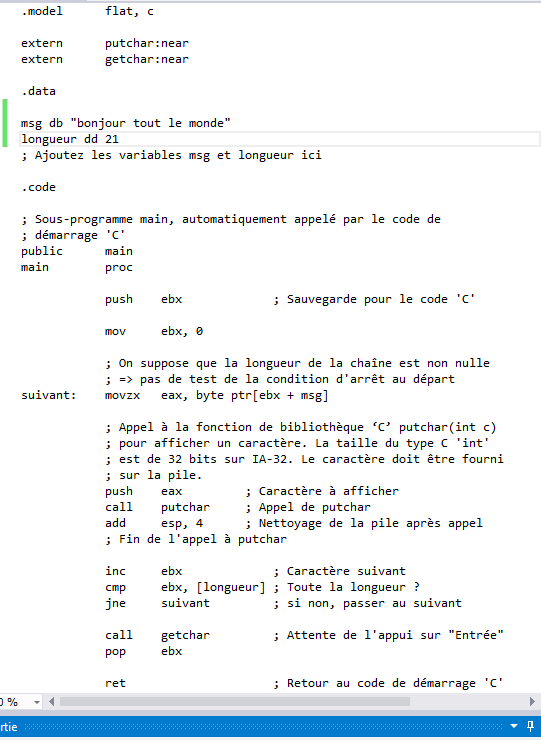
\includegraphics[width=8cm]{Capture5.PNG}
\caption{Programme "hello1"}
\end{figure}

\subsection{Chaîne de taille variable}

On modifie maintenant le premier code en "hello2" dans lequel la variable longueure n'est plus utilisée, à la place on définie la variable msg comme la chaine de caractère "bonjour tout le monde", terminée par un 0. 

Nous avons donc modifié le programme pour qu'il affiche toujours correctement le contenu de msg. Pour cela on garde ebx qui nous sert toujours de variable permettant de parcourir chaque caractère du message à afficher. Mais la comparaison se fait entre eax et 0 en effet si eax est égal à 0 cela signifie qu'on est arrivé à la fin du message (cela est valable car la chaîne message ne contient pas de caractère 0). 

L'algorithme implémenté correspond donc à un while(msg[ebx] != 0)



\begin{figure}[h]
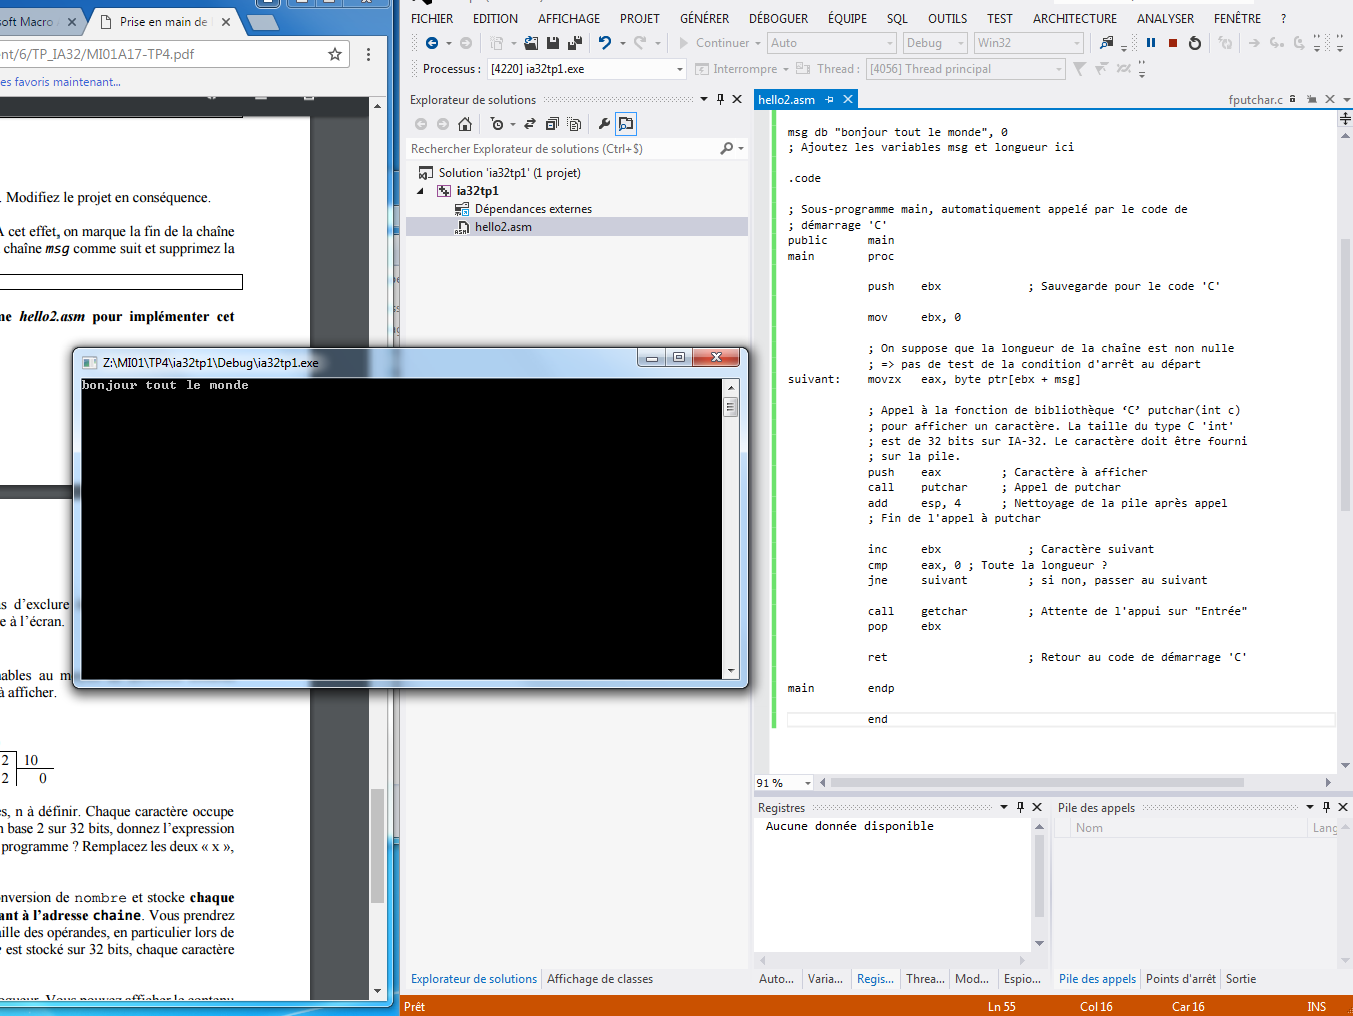
\includegraphics[width=15cm]{Capture4.PNG}
\caption{Programme "hello2"}
\end{figure}

\section{Exercice : conversion et afficahge de nombres}

Dans ce programme on cherche à convertir et afficher des nombres en différentes bases. 
Pour cela on utiliser une chaine de caractère de taille n pour stocker la conversion de nombre. Sachant nombre exprimé en base 2 sur 32 bits, le nombre max de bits utiles pour pouvoir écrire le résultat de nombre est donc 10. (car le résultat de $2^{32}$ s'écrit sur 10 chiffres, il faut donc une chaîne de 10 caractères). 



En base 35,  95c8ah est égale à 480724667

\end{document}
